%% ------------------------------------------------------------------------- %%
\chapter{Coreografias de serviços web}
\label{cap:servicos}

Neste capítulo descreveremos os conceitos básicos sobre a utilização e composição de serviços web, com foco nas coreografias.

\section{Serviços}
\label{sec:servicos}

Serviços são entidades autônomas e independentes de plataforma, que podem ser descritas, publicadas, encontradas e compostas~\cite{Papazoglou2007State}. O conceito de serviço é oriundo do conceito de \emph{componente}.

Componentes de software foram idealizados para que sistemas fossem construídos com ``blocos'' fornecidos por terceiros~\cite{McIlroy1968MassProduced}. Esses blocos teriam interfaces bem definidas e, com isso, seriam conectáveis entre si, sem que o desenvolvedor precisasse entender sobre a implementação desses blocos. Um exemplo bem conhecido de padronização de sistemas baseados em componentes é o Common Object Request Broker Architecture (CORBA). A especificação CORBA~\cite{CORBA1995} define objeto como uma ``entidade encapsulada e identificável que fornece um ou mais serviços que podem ser requisitados por um cliente'', o que corresponde ao conceito de componente. Ainda na especificação CORBA, uma interface é definida como uma ``descrição do conjunto de possíveis operações que um cliente pode requisitar para um objeto por essa interface''. Uma interface de um componente CORBA é concretamente descrita utilizando-se a Interface Description Language (IDL). \fabio{Livro básico de componentes:
 QA754.4 S999c; Procurar CORBA componente model}

\leo{Gancho entre componentes e serviços (serviços são uma sub-classe de componentes)}

Neste trabalho utilizaremos os termos ``serviço'' e ``serviço web'' de forma equivalentes, assim como feito por outros autores~\cite{Watson2006Dynasoar}. Daremos preferência ao termo ``serviço web'' para evitar os significados mais gerais que a palavra ``serviço'' pode assumir. Exceção poderá haver quando estivermos descrevendo trabalhos de terceiros que utilizam o termo ``serviço'' com algum significado mais amplo que o de ``serviço web''.

Um ponto de acesso (endpoint) de um serviço web é uma entidade referenciável para a qual envia-se mensagens construídas de acordo com a especificação do serviço~\cite{W3C2004Addressing}. Um ponto de acesso é referenciado por uma URI (\emph{Uniform Resource Identifier}) que possibilita o acesso a esse serviço pela Internet. Assim como Smith e Murray~\cite{Smith2010Evolution}, também utilizaremos a palavra serviço como simplificação para o ponto de acesso do serviço. 

As tecnologias mais utilizadas atualmente para a implementação de serviços são \emph{SOAP} e \emph{REST}. Os serviços SOAP utilizam um conjunto específico de protocolos definidos pela W3C. As mensagens trocadas pelos serviços SOAP possuem uma estrutura (envelope) encapsulada em mensagens HTTP, protocolo utilizado como um meio de transporte. Já os serviços REST utilizam o HTTP como protocolo de aplicação, utilizando assim diretamente os princípios arquiteturais que são utilizados para explicar a alta escalabilidade do protocolo HTTP e da própria World Wide Web~\cite{Pautasso2008Restful}. 

O W3C chama os serviços SOAP como ``serviços web'', fornecendo a seguinte definição: ``serviços web possibilitam a comunicação interoperável entre máquinas pela rede, utilizando padrões abertos para a troca de mensagens e descrição da interface dos serviços~\cite{W3C2004WS}''. Na prática, a única diferença dos serviços REST para essa definição é que em REST não se exige a descrição do serviço em linguagem legível por máquina, embora isso seja possível com a WADL~\cite{WADL2006}. Além disso, nessa definição da W3C também poderiam ser enquadradas outras tecnologias como CORBA. 

Serviços SOAP descrevem suas interfaces com a Web Service Descritption Language (WSDL), interagem entre si pela troca de mensagens SOAP e são publicados e descobertos em repositórios UDDI. Uma interface de um serviço web descrita em WSDL é um arquivo XML com uma estrutura padronizada, o que possibilita a outros sistemas analisarem as possíveis formas de interação com esse serviço. Mensagens SOAP também são estruturadas em XML, sendo normalmente enviadas no corpo de requisições e respostas HTTP. O envelope de uma mensagem SOAP codifica a requisição ou resposta à operação de um serviço web, descrevendo também os tipos de dados e valores envolvidos na operação. 

Além dos padrões mencionados (WSDL, SOAP, UDDI), há vários outros padrões que formam o conjunto chamado de WS-*, que inclui especificações para a realização de transações entre serviços, troca de endereços de serviços, composição de processos de negócios e muitos outros. O uso desse conjunto de padrões de forma integrada se relaciona com a criação de Arquiteturas Orientadas a Serviços (SOA). De acordo com Papazoglou~\cite{Papazoglou2007State}, SOA é uma forma de projetar sistemas que forneçam serviços com interfaces publicadas que possam ser descobertas, de modo que funcionalidades da aplicação sejam reutilizáveis como serviços por outras aplicações ou serviços em um ambiente distribuído. 

Serviços REST utilizam como \emph{interface uniforme} os verbos do protocolo HTTP (GET, POST, PUT e DELETE) e se comunicam fazendo uso do protocolo HTTP como protocolo de aplicação. Serviços REST não estão presos a um formato de troca de mensagens, pois a cada mensagem o formato é descrito por um tipo MIME (ex: xml, json, png, txt). Em REST, também não existe a noção de registro de serviços, pois a identificação de recursos por URIs e o uso de hyperlinks nas próprias mensagens REST possibilitam que os serviços necessários para a aplicação sejam encontrados~\cite{Pautasso2008Restful}.

Ainda segundo Pautasso~\cite{Pautasso2008Restful}, serviços REST são considerados ``mais simples'' do que serviços web porque fazem uso de padrões já bem estabelecidos, como HTTP, XML, URI e MIME, para os quais já existe uma ampla infraestrutura implantada. Um exemplo disso, é que é possível testar alguns serviços REST apenas com um navegador comum. Parte da escalabilidade atribuída a serviços REST também vem desse uso de padrões bem estabelecidos, pois os \emph{caches} implementados pelos servidores web se tornam automaticamente caches para serviços REST~\cite{Tong2010CXF}.

Apesar das vantagens apresentadas dos serviços REST, serviços que utilizam a tecnologia WS-* ainda são mais propensos a uma série de manipulações automatizadas que se tornam mais difíceis nos serviços REST, como por exemplo a geração automatizada de clientes para uma dada linguagem de programação. Isso se deve principalmente pelo alto nível de padronização da tecnologia WS-* e pela existência de interfaces bem definidas e processáveis por software (WSDL). 

\section{Composições de serviços web}
\label{sec:composicoes}

Serviços são compostos para implementar processos de negócios mais sofisticados~\cite{Papazoglou2007State}. Processos de negócio são sequências bem definidas de passos computacionais executados de uma maneira coordenada~\cite{Alonso2002Atomicity}. A principal tecnologia para a implementação de processos de negócios são os sistemas de gerenciamento de workflow~\cite{Agostini2000Improving}. Um workflow é a automação, total ou parcial, de um processo de negócio, no qual documentos, informações ou tarefas são passados de um participante (humano ou não) para outros, de acordo com um conjunto de regras de procedimento~\cite{WorkflowCoalition1999}. Segundo Casati et al.~\cite{Casati1998Workflow}, workflows são compostos de \emph{tarefas}, unidades de trabalho a serem desempenhadas por agentes humanos ou automatizados e \emph{conectores}, que definem a ordem em que as tarefas devem ser executadas, o que também é denominado \emph{fluxo de controle}. Sincronizações de execuções concorrentes também são especificadas por controladores chamados ``joins'' e ``forks''. Quando uma tarefa é desempenhada por um agente automatizado, o gerenciador de workflow normalmente realiza a invocação de um serviço web, que é esse agente automatizado que participa do processo de negócio. Um exemplo de linguagem para a criação de processo de negócio a partir da composição de serviços web é a WS-BPEL~\cite{BPEL2007}.

O modelo de composição de serviços web no qual temos um coordenador central que coordenada o fluxo de controle da composição é denominado \emph{orquestração}~\cite{Nanda2004Decentralizing}. O coordenador central é chamado de \emph{orquestrador}. No caso em que processos de negócios são executados por sistemas gerenciadores de workflows, o orquestrador é o próprio sistema de workflow.

Outro modelo de composição de serviços web é o de \emph{coreografia}, no qual o conhecimento sobre o fluxo de controle é distribuído entre os participantes, ou seja, cada serviço envolvido na composição sabe quando executar suas operações e com quais outros serviços interagir, sem que seja preciso um controle centralizado~\cite{Barker2009Choreographing}. 

Exemplos de linguagens e notações de descrição de coreografias são WSCI~\cite{WSCI2002}, WS-CDL~\cite{WSCDL2005} e BPMN2~\cite{BPMN2011}. Essas linguagens e notações descrevem sequências e restrições nas trocas de mensagens efetuadas pelos participantes da coreografia sob uma perspectiva global. Essa descrição é vista como um contrato de negócios entre duas ou mais organizações~\cite{BPMN2011}. Apesar da perspectiva global, como ressalta a especificação do BPMN2, uma coreografia não possui um controle de execução centralizado e participantes não compartilham um espaço de dados global. Dessa forma, um participante conhece o estado de outro participante apenas pela observação de seu comportamento externo, que consiste nas trocas de mensagens efetuadas~\cite{BPMN2011}.

Cada participante da coreografia pode ter o seu comportamento modelado por uma linguagem de orquestração, que no caso do BPMN2 corresponde a um diagrama de processo. Dessa forma, uma coreografia pode também ser modelada como um conjunto de orquestrações distribuídas que interagem entre si, de forma que apenas os orquestradores precisam estar cientes de condições impostas pela coreografia~\cite{Poulin2011Collaboration}.
% parece que Rinderle também corrobora com isso

Um diagrama BPMN2 de coreografia especifica passos na execução da coreografia, que são denominados \emph{atividades}, e que consistem na troca de mensagens entre \emph{participantes}~\cite{BPMN2011}. Uma atividade pode ocorrer entre entidades participantes (ex: Magalhães Viagens realiza compra de passagem aérea da Nimbus Airline) ou entre \emph{papéis} de participantes (ex: uma Agência de Viagem requisita pedido de entrega a uma Companhia Aérea). Dizemos que dois serviços desempenham o mesmo papel se fornecem funcionalidades equivalentes. O BPMN2 distingue um dos participantes de uma atividade como o participante iniciador, que é aquele que envia a mensagem ao outro participante. O participante iniciador é também denominado cliente ou consumidor, enquanto que o outro participante é também denominado provedor. O diagrama BPMN da Figura~\ref{fig:bpmn1} ilustra os elementos explicados em um exemplo de uma pequena coreografia com apenas dois serviços.

\begin{figure}[!h]
  \centering
  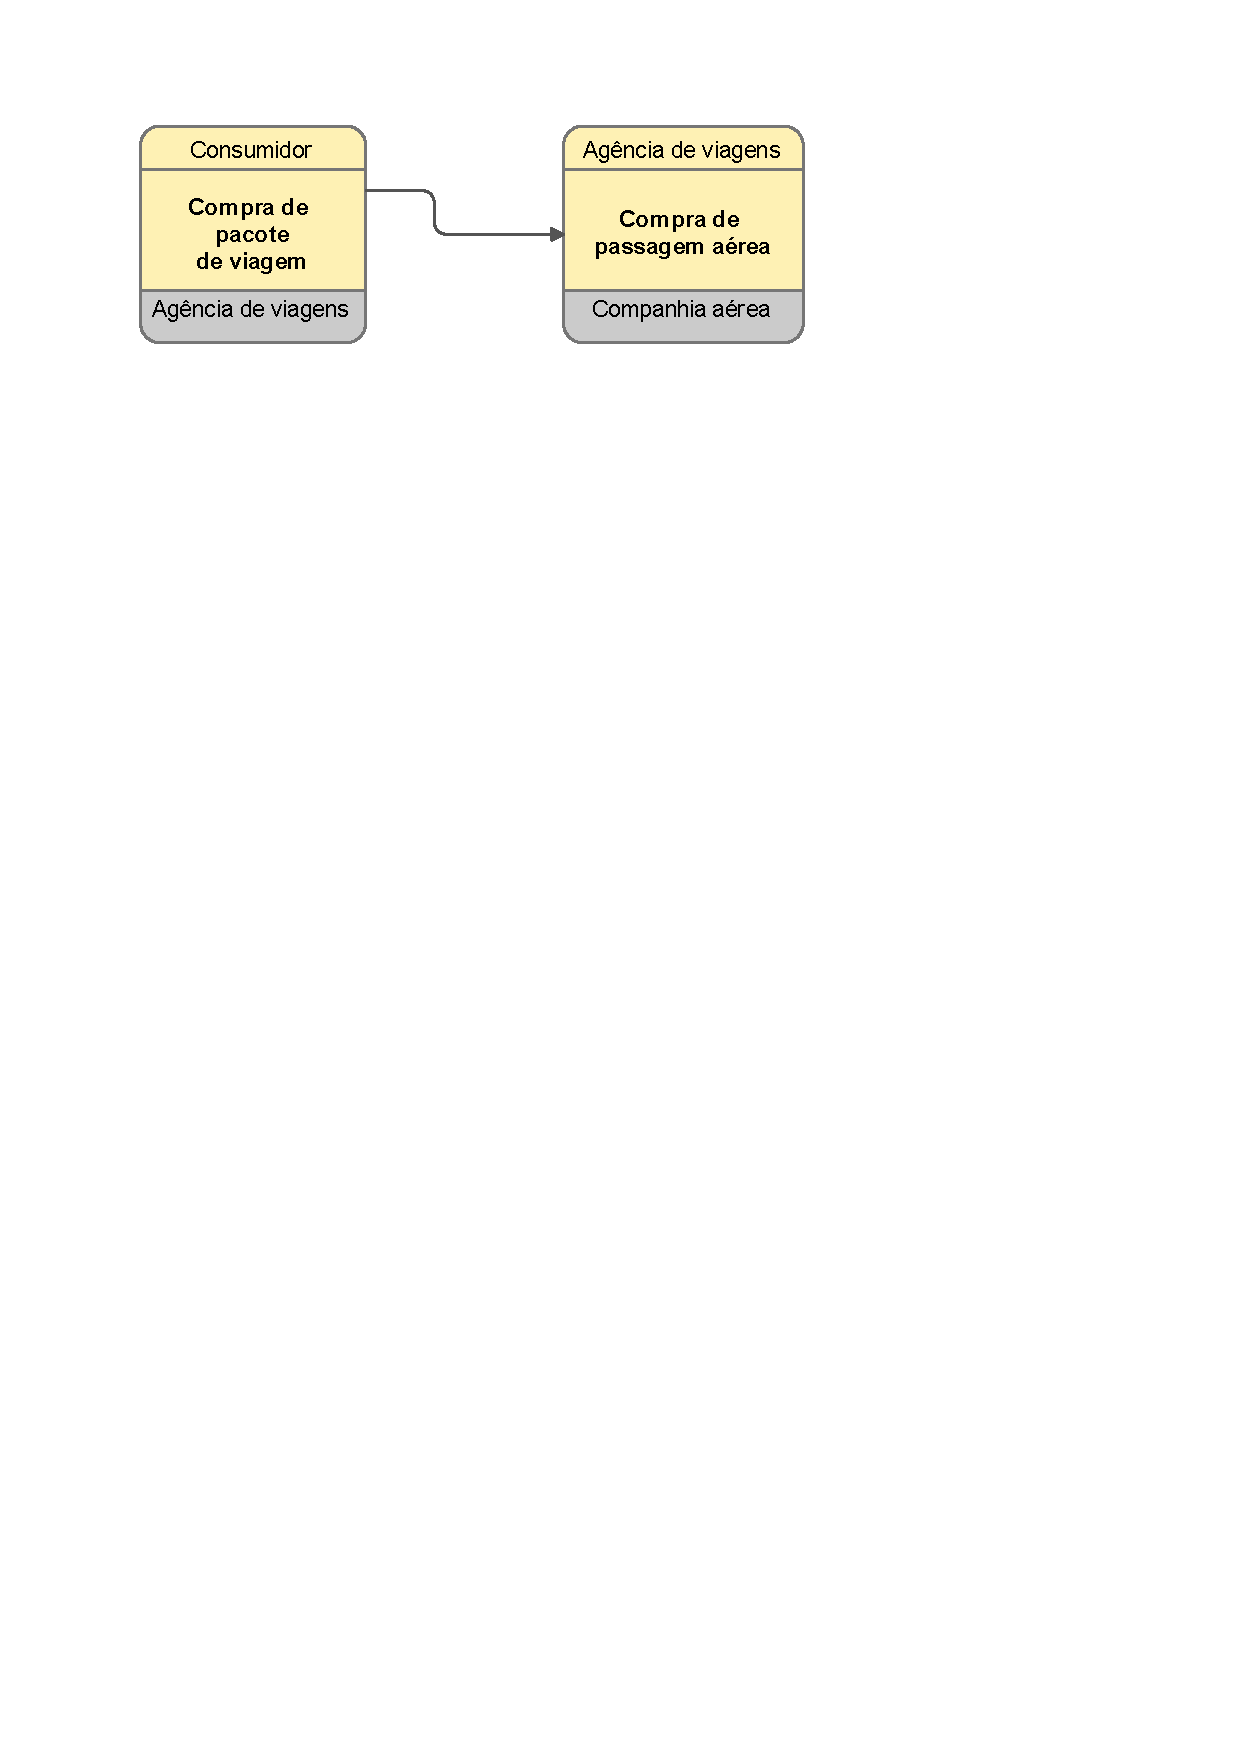
\includegraphics[width=.60\textwidth]{bpmn1.pdf} 
  \caption{Exemplo de uma pequena coreografia de serviços em notação BPMN2.}
  \label{fig:bpmn1} 
\end{figure}

%\begin{figure}[!h]
%  \centering
%  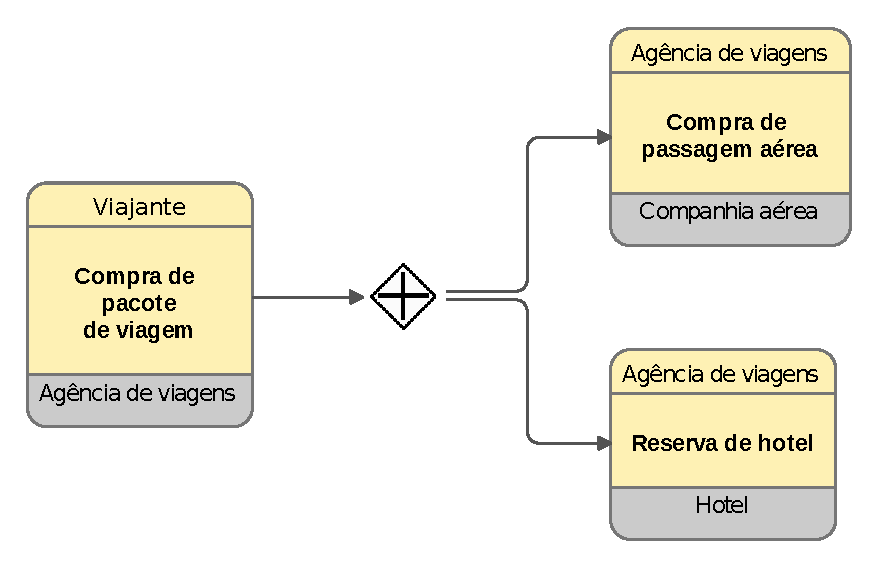
\includegraphics[width=.60\textwidth]{bpmn2.pdf} 
%  \caption{Outro exemplo de diagrama BPMN2, ligeiramente mais sofisticado.}
%  \label{fig:bpmn2} 
%\end{figure}

Serviços podem ser projetados para participarem de uma determinada composição, mas também é possível que uma composição seja projetada para utilizar serviços já existentes. No segundo caso, é necessária a criação de serviços de coordenação que fazem com que serviços já existentes, não-cientes da composição, se comuniquem adequadamente~\cite{Autili2013Synthesis}. 

Em artigos acadêmicos também é comum a modelagem de coreografias com notações mais formais, tais como álgebras de processos, redes de Petri e autômatos. Essas notações possibilitam aos autores realizarem simulações e identificarem propriedades, como a verificação da consistência da evolução dinâmica de coreografias~\cite{Cicirelli2010Dynamically}. Em nosso trabalho, como estaremos preocupados em viabilizar a execução de coreografias, adotaremos como modelagem de referência a notação BPMN2, que é um padrão de indústria.

